\documentclass[12pt,a4paper]{article}

%====================================================
% ENCODING & LANGUAGE
%====================================================
\usepackage[T1]{fontenc}
\usepackage[utf8]{inputenc}
\usepackage[english]{babel}

%====================================================
% FONT
%====================================================
\usepackage{mathptmx}

%====================================================
% MATH
%====================================================
\usepackage{amsmath}
\usepackage{amsfonts}
\usepackage{amssymb}

%====================================================
% GRAPHICS
%====================================================
\usepackage{graphicx}
\graphicspath{{./image/}}

%====================================================
% TABLES
%====================================================
\usepackage[table]{xcolor}
\usepackage{float}
\usepackage{booktabs}
\usepackage{longtable}
\usepackage{tabularx}
\usepackage{array}
\usepackage{multirow}
\usepackage{caption}
\usepackage{enumitem}

%====================================================
% PAGE LAYOUT
%====================================================
\usepackage{geometry}
\geometry{
    top=2.5cm,
    bottom=2.5cm,
    left=3.0cm,
    right=2.0cm,
    headheight=14pt
}

\setlength{\emergencystretch}{3em}

%====================================================
% SPACING
%====================================================
\usepackage{setspace}
\onehalfspacing

\usepackage{indentfirst}
\setlength{\parindent}{1.27cm}
\setlength{\parskip}{6pt}

%====================================================
% COLORS
%====================================================
\definecolor{fptred}{RGB}{192,0,0}
\definecolor{fptBlue}{RGB}{0,0,139}
\definecolor{fptOrange}{RGB}{255,140,0}
\definecolor{headerbg}{RGB}{242,226,204}

%====================================================
% SECTION FORMAT
%====================================================
\usepackage{titlesec}

\setcounter{secnumdepth}{3}
\setcounter{tocdepth}{3}

\titleformat{\section}
  {\normalfont\Large\bfseries}
  {\thesection}{0.8em}{}

\titleformat{\subsection}
  {\normalfont\large\bfseries}
  {\thesubsection}{0.8em}{}

\titleformat{\subsubsection}
  {\normalfont\normalsize\bfseries}
  {\thesubsubsection}{0.8em}{}

\titlespacing*{\section}{0pt}{2.4ex plus 1ex minus .2ex}{1.2ex plus .2ex}
\titlespacing*{\subsection}{0pt}{1.8ex plus .8ex minus .2ex}{0.8ex plus .2ex}
\titlespacing*{\subsubsection}{0pt}{1.4ex plus .6ex minus .2ex}{0.6ex plus .2ex}

%====================================================
% HEADER & FOOTER
%====================================================
\usepackage{fancyhdr}

\pagestyle{fancy}
\fancyhf{}
\fancyhead[L]{\small\textit{FREVIA --- Project Management Plan}}
\fancyhead[R]{\small\leftmark}
\fancyfoot[C]{\small\thepage}
\renewcommand{\headrulewidth}{0.4pt}
\renewcommand{\footrulewidth}{0pt}

\fancypagestyle{plain}{
  \fancyhf{}
  \fancyfoot[C]{\small\thepage}
  \renewcommand{\headrulewidth}{0pt}
}

%====================================================
% CAPTIONS
%====================================================
\captionsetup{
    font=small,
    labelfont=bf,
    justification=centering,
    skip=6pt
}

%====================================================
% TABLE OF CONTENTS
%====================================================
\usepackage{tocloft}

\renewcommand{\cftsecleader}{\cftdotfill{\cftdotsep}}
\renewcommand{\cftsubsecleader}{\cftdotfill{\cftdotsep}}
\renewcommand{\cftsubsubsecleader}{\cftdotfill{\cftdotsep}}

\renewcommand{\cftsecfont}{\bfseries}
\renewcommand{\cftsecpagefont}{\bfseries}

\setlength{\cftbeforesecskip}{6pt}
\setlength{\cftbeforesubsecskip}{2pt}

%====================================================
% HYPERLINKS
%====================================================
\usepackage{hyperref}

\hypersetup{
    colorlinks=true,
    linkcolor=black,
    citecolor=black,
    filecolor=black,
    urlcolor=blue,
    pdftitle={FREVIA Project Management Plan},
    pdfauthor={Group Frevia}
}

%====================================================
% CUSTOM COLUMN TYPES
%====================================================
\newcolumntype{L}[1]{>{\raggedright\arraybackslash}p{#1}}
\newcolumntype{C}[1]{>{\centering\arraybackslash}p{#1}}
\newcolumntype{R}[1]{>{\raggedleft\arraybackslash}p{#1}}

%====================================================
% DOCUMENT
%====================================================
\begin{document}

%====================================================
% COVER PAGE
%====================================================
\pagenumbering{roman}
\begin{titlepage}
    \centering
    \thispagestyle{empty}
    \hypersetup{pageanchor=false}

    
\includegraphics[width=0.38\textwidth]{image/school_logo.png}
    \vspace{0.9cm}

    {\Huge\bfseries\textcolor{fptred}{FPT UNIVERSITY}}\\[0.45cm]
    {\LARGE\bfseries\textcolor{fptred}{Project Management Plan}}\\[0.35cm]

    {\color{fptOrange}\rule{0.82\textwidth}{1.2pt}}
    \vspace{0.5cm}

    {\Huge\bfseries\textcolor{fptred}{FREVIA}}\\[0.2cm]
    {\large Verified Freelance Marketplace Platform}\\[1.4cm]

    \renewcommand{\arraystretch}{1.65}
    \arrayrulecolor{fptOrange}
    \begin{tabular}{|m{4.3cm}|m{7.7cm}|}
        \hline
        \multicolumn{2}{|c|}{\Large\bfseries\textcolor{fptBlue}{Group Frevia}} \\
        \hline
        \multirow{5}{*}{\centering\bfseries Group Members}
            & Pham Kha Vy -- CE182254 \\
            & Nguyen Tien Thuan -- CE181024 \\
            & Tran Phat Tai -- CE181632 \\
            & Vo Nhut Tin -- CE180619 \\
            & Nguyen Lu Nhat Huy -- CE181196 \\
        \hline
        \textbf{Supervisor} & Mrs. Cao Hong Nga \\
        \hline
        \textbf{External Supervisor} & \\
        \hline
        \textbf{Capstone Project Code} & SEP490\_04 \\
        \hline
    \end{tabular}
    \vfill

    {\bfseries Can Tho, October 2026}
    \hypersetup{pageanchor=true}
\end{titlepage}


%====================================================
% TABLE OF CONTENTS
%====================================================
\newpage
\renewcommand{\contentsname}{\fontsize{20}{24}\selectfont\bfseries Table of Contents}
\tableofcontents
\newpage
\pagenumbering{arabic}

%====================================================
% MAIN CONTENT
%====================================================
\section{Overview}
    \subsection{Scope \& Estimation}
    The work breakdown below is the basis for sprint planning. Each row is a SMAR (Specific, Measurable, Achievable, Relevant) item that can be demonstrated at the end of the sprint in which it is scheduled, and the identifier in the second column is the reference used by the task board, the review checklist, and the test cases. Complexity is rated Low, Medium or High according to technical uncertainty and integration risk rather than to effort alone; effort is estimated in man-days and rounded to whole days. Module header rows carry no estimate because their effort is already distributed across the items beneath them.

\setlength\LTleft{0pt}\setlength\LTright{0pt}

\begin{longtable}{|
c|
c|
>{\raggedright\arraybackslash}p{6.2cm}|
>{\centering\arraybackslash}p{1.8cm}|
>{\centering\arraybackslash}p{1.7cm}|
>{\centering\arraybackslash}p{1.8cm}|}

\hline
\rowcolor{fptOrange} \textbf{No} & \textbf{\#} & \textbf{SMAR Item} & \textbf{Iteration Code} & \textbf{Complexity} & \textbf{Est. Effort (man days)} \\
\hline
\endfirsthead

\hline
\rowcolor{fptOrange} \textbf{No} & \textbf{\#} & \textbf{SMAR Item} & \textbf{Iteration Code} & \textbf{Complexity} & \textbf{Est. Effort (man days)} \\
\hline
\endhead

\hline
\endfoot

\hline\hline
\endlastfoot

% ========== SPRINT 1: IDENTITY, ACCESS, PROFILES, JOBS ==========

1  & & \textbf{Authentication} & & -- & -- \\
2  & 1.1 & Register with email one-time-code verification & \multirow{8}{*}{Sprint 1} & Medium & 3 \\
3  & 1.2 & Google OAuth sign-in and account linking & & Medium & 3 \\
4  & 1.3 & Login and logout with JWT issuance & & Low & 2 \\
5  & 1.4 & Refresh token rotation and persisted sessions & & Medium & 3 \\
6  & 1.5 & Password reset through a one-time code & & Low & 2 \\
7  & 1.6 & Password change from account settings & & Low & 1 \\
8  & 1.7 & Multi-role membership, join role and role switching & & Medium & 3 \\
9  & 1.8 & Account profile with avatar and cover upload & & Medium & 3 \\
\hline

10 & & \textbf{Authorization and Administration} & & -- & -- \\
11 & 1.9 & Permission model bound to method, path and module & \multirow{7}{*}{Sprint 1} & Medium & 3 \\
12 & 1.10 & Permission guard and public route decorator & & Medium & 3 \\
13 & 1.11 & Administrative role management & & Medium & 2 \\
14 & 1.12 & Administrative permission assignment & & Medium & 2 \\
15 & 1.13 & Administrative user creation and update & & Medium & 2 \\
16 & 1.14 & Account ban and unban & & Low & 1 \\
17 & 1.15 & Session listing, detail and revocation & & Medium & 2 \\
\hline

18 & & \textbf{Profile and Portfolio} & & -- & -- \\
19 & 1.16 & Freelancer profile with education and certifications & \multirow{8}{*}{Sprint 1} & Medium & 3 \\
20 & 1.17 & Work experience entries with dates and description & & Low & 2 \\
21 & 1.18 & Client profile with company information & & Low & 1 \\
22 & 1.19 & Skills with proficiency level and suggestions & & Medium & 2 \\
23 & 1.20 & Portfolio items with technologies and cover image & & Medium & 3 \\
24 & 1.21 & Social link management & & Low & 1 \\
25 & 1.22 & Profile completion and strength scoring & & Medium & 2 \\
26 & 1.23 & Profile revision submission and approval & & Medium & 3 \\
\hline

27 & & \textbf{Curriculum Vitae Handling} & & -- & -- \\
28 & 1.24 & CV upload and secure storage & \multirow{3}{*}{Sprint 1} & Medium & 2 \\
29 & 1.25 & CV preview and download & & Low & 1 \\
30 & 1.26 & CV replacement and deletion & & Low & 1 \\
\hline

31 & & \textbf{Job Marketplace} & & -- & -- \\
32 & 1.27 & Job creation with budget, deadline, skills and categories & \multirow{9}{*}{Sprint 1} & Medium & 3 \\
33 & 1.28 & Job editing and deletion with ownership validation & & Medium & 2 \\
34 & 1.29 & Job status lifecycle & & Medium & 2 \\
35 & 1.30 & Client job list and detail & & Medium & 2 \\
36 & 1.31 & Public job search with keyword matching & & Medium & 2 \\
37 & 1.32 & Public job filters by category, skill and budget range & & Medium & 3 \\
38 & 1.33 & Job detail page with contextual actions & & Medium & 2 \\
39 & 1.34 & Job category browsing & & Low & 1 \\
40 & 1.35 & Unique, stable slug generated for every published job & & Low & 2 \\
\hline

41 & & \textbf{Bookmarks and Saved Search} & & -- & -- \\
42 & 1.36 & Job bookmark save, remove and status & \multirow{4}{*}{Sprint 1} & Low & 1 \\
43 & 1.37 & Bookmarked job list & & Low & 1 \\
44 & 1.38 & Saved search creation and listing & & Medium & 2 \\
45 & 1.39 & Saved search update and deletion & & Medium & 2 \\
\hline

46 & & \textbf{Community Forum Foundation} & & -- & -- \\
47 & 1.40 & Forum category listing & \multirow{5}{*}{Sprint 1} & Low & 1 \\
48 & 1.41 & Forum post creation with rich text and tags & & Medium & 3 \\
49 & 1.42 & Forum post listing, search and detail & & Medium & 2 \\
50 & 1.43 & Comments, likes and reporting & & Medium & 3 \\
51 & 1.44 & Administrative approval of pending posts & & Low & 1 \\
\hline

52 & & \textbf{Identity Verification Capture} & & -- & -- \\
53 & 1.45 & Identity document upload with front and back images & \multirow{4}{*}{Sprint 1} & Medium & 3 \\
54 & 1.46 & Selfie capture and liveness frame submission & & Medium & 3 \\
55 & 1.47 & AI verification request, timeout and result handling & & High & 5 \\
56 & 1.48 & Verification status display & & Medium & 2 \\
\hline

% ========== SPRINT 2: PROPOSALS, CONTRACTS, MILESTONES ==========

57 & & \textbf{Proposal Management} & & -- & -- \\
58 & 2.1 & Proposal creation with bid, duration and cover letter & \multirow{9}{*}{Sprint 2} & Medium & 2 \\
59 & 2.2 & Proposal attachments & & Low & 1 \\
60 & 2.3 & Save proposal as draft & & Medium & 2 \\
61 & 2.4 & Proposal editing & & Medium & 2 \\
62 & 2.5 & Proposal withdrawal & & Low & 1 \\
63 & 2.6 & Proposal expiry handling & & Medium & 2 \\
64 & 2.7 & Freelancer proposal list and filters & & Low & 2 \\
65 & 2.8 & Client proposal list for a job & & Low & 2 \\
66 & 2.9 & Proposal detail with applicant profile & & Low & 1 \\
\hline

67 & & \textbf{Hiring Decision} & & -- & -- \\
68 & 2.10 & Accept proposal and create contract & \multirow{3}{*}{Sprint 2} & Medium & 3 \\
69 & 2.11 & Reject proposal & & Low & 1 \\
70 & 2.12 & Position count enforcement for multiple hiring & & Medium & 2 \\
\hline

71 & & \textbf{Contract Management} & & -- & -- \\
72 & 2.13 & Contract generation from an accepted proposal & \multirow{6}{*}{Sprint 2} & Medium & 3 \\
73 & 2.14 & Contract list and detail for both parties & & Medium & 2 \\
74 & 2.15 & Dual contract signing & & Medium & 3 \\
75 & 2.16 & Platform fee recording and contract total & & Medium & 2 \\
76 & 2.17 & Contract completion & & Medium & 2 \\
77 & 2.18 & Contract cancellation & & Medium & 2 \\
\hline

78 & & \textbf{Milestone Management} & & -- & -- \\
79 & 2.19 & Milestone list and detail & \multirow{8}{*}{Sprint 2} & Low & 1 \\
80 & 2.20 & Milestone creation & & Medium & 2 \\
81 & 2.21 & Milestone editing & & Medium & 2 \\
82 & 2.22 & Milestone deletion and start-in-progress transition & & Low & 1 \\
83 & 2.23 & Submission with message and external links & & Medium & 2 \\
84 & 2.24 & Submission file upload and removal & & Medium & 2 \\
85 & 2.25 & Change request with message and due date & & Medium & 2 \\
86 & 2.26 & Submission approval and completion trigger & & Medium & 3 \\
\hline

87 & & \textbf{Milestone Files} & & -- & -- \\
88 & 2.27 & Milestone file listing & \multirow{3}{*}{Sprint 2} & Low & 1 \\
89 & 2.28 & Milestone file upload and type validation & & Medium & 2 \\
90 & 2.29 & Milestone file deletion & & Low & 1 \\
\hline

91 & & \textbf{Milestone Progress} & & -- & -- \\
92 & 2.30 & Start a milestone (pending to in progress) & \multirow{2}{*}{Sprint 2} & Low & 1 \\
93 & 2.31 & Milestone state display in the contract view & & Low & 1 \\
\hline

94 & & \textbf{Contract Shared Files} & & -- & -- \\
95 & 2.32 & Shared file upload & \multirow{2}{*}{Sprint 2} & Medium & 2 \\
96 & 2.33 & Shared file listing and deletion & & Low & 1 \\
\hline

97 & & \textbf{Review and Rating} & & -- & -- \\
98 & 2.34 & Contract review with overall rating and breakdown & \multirow{6}{*}{Sprint 2} & Medium & 3 \\
99 & 2.35 & Review editing and deletion & & Low & 1 \\
100 & 2.36 & Contract review listing & & Low & 1 \\
101 & 2.37 & Review detail & & Low & 1 \\
102 & 2.38 & Review response creation & & Low & 1 \\
103 & 2.39 & Review response update and deletion & & Low & 1 \\
\hline

% ========== SPRINT 3: COMMUNICATION, NOTIFICATIONS, ADMINISTRATION ==========

104 & & \textbf{Real-time Messaging} & & -- & -- \\
105 & 3.1 & Conversation model and conversation list & \multirow{9}{*}{Sprint 3} & Medium & 2 \\
106 & 3.2 & Starting a conversation & & Medium & 2 \\
107 & 3.3 & Socket authentication and gateway setup & & Medium & 3 \\
108 & 3.4 & Sending text messages & & Medium & 2 \\
109 & 3.5 & File attachment messages & & Medium & 2 \\
110 & 3.6 & Read receipts & & Low & 1 \\
111 & 3.7 & Typing indicator & & Low & 1 \\
112 & 3.8 & Message deletion & & Low & 1 \\
113 & 3.9 & Conversation pinning, hiding and unread count & & Medium & 2 \\
\hline

114 & & \textbf{Notification Centre} & & -- & -- \\
115 & 3.10 & Notification creation from domain events & \multirow{5}{*}{Sprint 3} & Medium & 2 \\
116 & 3.11 & Notification list with typed entries & & Medium & 2 \\
117 & 3.12 & Unread count and badge & & Low & 1 \\
118 & 3.13 & Mark as read and mark all as read & & Low & 1 \\
119 & 3.14 & Notification deletion & & Low & 1 \\
\hline

120 & & \textbf{Saved Search Refinement} & & -- & -- \\
121 & 3.15 & Saved search filters by category and budget & \multirow{4}{*}{Sprint 3} & Low & 1 \\
122 & 3.16 & Saved search order and pagination & & Low & 1 \\
123 & 3.17 & Saved search naming and rename & & Low & 1 \\
124 & 3.18 & Saved search application to the job search screen & & Low & 1 \\
\hline

125 & & \textbf{Session Management} & & -- & -- \\
126 & 3.19 & Active session list with device and IP address & \multirow{3}{*}{Sprint 3} & Medium & 2 \\
127 & 3.20 & Session detail & & Low & 1 \\
128 & 3.21 & Session revocation & & Low & 1 \\
\hline

129 & & \textbf{Permission Administration} & & -- & -- \\
130 & 3.22 & Permission creation & \multirow{3}{*}{Sprint 3} & Medium & 2 \\
131 & 3.23 & Permission listing and editing & & Low & 1 \\
132 & 3.24 & Permission deletion and role binding review & & Low & 1 \\
\hline

133 & & \textbf{User Administration} & & -- & -- \\
134 & 3.25 & Administrative user list with search and filters & \multirow{8}{*}{Sprint 3} & Medium & 2 \\
135 & 3.26 & Administrative user detail & & Low & 1 \\
136 & 3.27 & Administrative user creation & & Medium & 2 \\
137 & 3.28 & Administrative user update & & Medium & 2 \\
138 & 3.29 & Ban and unban accounts & & Low & 1 \\
139 & 3.30 & Administrative client profile editing & & Low & 1 \\
140 & 3.31 & Administrative freelancer profile editing & & Low & 1 \\
141 & 3.32 & Skill catalogue lookup for administrative forms & & Low & 1 \\
\hline

142 & & \textbf{Profile Revision Review} & & -- & -- \\
143 & 3.33 & Revision queue with pending and approved filters & \multirow{3}{*}{Sprint 3} & Medium & 2 \\
144 & 3.34 & Comparison of proposed and current profile data & & Medium & 2 \\
145 & 3.35 & Approve or reject a revision & & Low & 1 \\
\hline

146 & & \textbf{Identity Verification Review} & & -- & -- \\
147 & 3.36 & Verification review queue & \multirow{3}{*}{Sprint 3} & Medium & 2 \\
148 & 3.37 & Document viewer with access control & & Low & 1 \\
149 & 3.38 & Verification decision and badge publication & & Medium & 2 \\
\hline

150 & & \textbf{Forum Categories} & & -- & -- \\
151 & 3.39 & Forum category creation & \multirow{4}{*}{Sprint 3} & Low & 1 \\
152 & 3.40 & Forum category listing and search & & Low & 1 \\
153 & 3.41 & Forum category editing & & Low & 1 \\
154 & 3.42 & Forum category deletion & & Low & 1 \\
\hline

155 & & \textbf{Forum Moderation} & & -- & -- \\
156 & 3.43 & AI moderation payload ingestion & \multirow{5}{*}{Sprint 3} & Medium & 2 \\
157 & 3.44 & Moderation queue with risk filters & & Medium & 2 \\
158 & 3.45 & Approve and reject actions from the queue & & Low & 1 \\
159 & 3.46 & Report handling and resolution & & Low & 1 \\
160 & 3.47 & Forum trash and restore & & Low & 1 \\
\hline

% ========== SPRINT 4: PAYMENTS AND DISPUTES ==========

161 & & \textbf{Stripe Connect Onboarding} & & -- & -- \\
162 & 4.1 & Express account onboarding link & \multirow{4}{*}{Sprint 4} & Medium & 3 \\
163 & 4.2 & Onboarding status synchronisation & & Medium & 2 \\
164 & 4.3 & Saved payment method listing & & Low & 1 \\
165 & 4.4 & Customer portal session & & Low & 1 \\
\hline

166 & & \textbf{Milestone Funding} & & -- & -- \\
167 & 4.5 & Platform fee PaymentIntent & \multirow{5}{*}{Sprint 4} & Medium & 3 \\
168 & 4.6 & Milestone funding PaymentIntent & & Medium & 3 \\
169 & 4.7 & Hosted Checkout Session for funding & & Medium & 2 \\
170 & 4.8 & Funding with a saved card & & Medium & 2 \\
171 & 4.9 & Funding state synchronisation & & Medium & 2 \\
\hline

172 & & \textbf{Release, Refund and Ledger} & & -- & -- \\
173 & 4.10 & Milestone release as a Stripe transfer & \multirow{4}{*}{Sprint 4} & High & 4 \\
174 & 4.11 & Refund processing & & Medium & 3 \\
175 & 4.12 & Dispute settlement with split payouts & & Medium & 3 \\
176 & 4.13 & Transaction ledger with type and status & & Medium & 2 \\
\hline

177 & & \textbf{Payment Webhooks} & & -- & -- \\
178 & 4.14 & Webhook endpoint with signature verification & \multirow{3}{*}{Sprint 4} & Medium & 3 \\
179 & 4.15 & PaymentIntent event handling & & Low & 1 \\
180 & 4.16 & Checkout Session event handling & & Low & 1 \\
\hline

181 & & \textbf{Dispute Management} & & -- & -- \\
182 & 4.17 & Dispute creation with claim evidence & \multirow{8}{*}{Sprint 4} & Medium & 3 \\
183 & 4.18 & Arbitration fee payment intent & & Medium & 2 \\
184 & 4.19 & Fee and response deadline handling & & Medium & 2 \\
185 & 4.20 & Dispute response with evidence & & Medium & 2 \\
186 & 4.21 & Dispute list and detail for participants & & Low & 1 \\
187 & 4.22 & Decision review request & & Medium & 2 \\
188 & 4.23 & Administrative decision with split and reasoning & & Medium & 3 \\
189 & 4.24 & Final decision and dispute closure & & Low & 1 \\
\hline

190 & & \textbf{Advertisement Banners} & & -- & -- \\
191 & 4.25 & Banner creation & \multirow{5}{*}{Sprint 4} & Low & 1 \\
192 & 4.26 & Banner listing & & Low & 1 \\
193 & 4.27 & Banner editing & & Low & 1 \\
194 & 4.28 & Banner deletion and activation window & & Low & 1 \\
195 & 4.29 & Public banner display by placement position & & Low & 1 \\
\hline

196 & & \textbf{Skill Catalogue} & & -- & -- \\
197 & 4.30 & Skill creation & \multirow{5}{*}{Sprint 4} & Low & 1 \\
198 & 4.31 & Skill listing and search & & Low & 1 \\
199 & 4.32 & Skill editing & & Low & 1 \\
200 & 4.33 & Skill soft deletion & & Low & 1 \\
201 & 4.34 & Skill restore & & Low & 1 \\
\hline

202 & & \textbf{Job Categories} & & -- & -- \\
203 & 4.35 & Category creation & \multirow{5}{*}{Sprint 4} & Low & 1 \\
204 & 4.36 & Category listing and search & & Low & 1 \\
205 & 4.37 & Category editing & & Low & 1 \\
206 & 4.38 & Category soft deletion & & Low & 1 \\
207 & 4.39 & Category restore and status toggle & & Low & 1 \\
\hline

% ========== SPRINT 5: EXTENSION, LOCALISATION, HARDENING ==========

208 & & \textbf{AI Curriculum Vitae Analysis} & & -- & -- \\
209 & 5.1 & AI service client with timeout and retry policy & \multirow{4}{*}{Sprint 5} & Medium & 3 \\
210 & 5.2 & Skill suggestion parsing and validation & & Medium & 2 \\
211 & 5.3 & Suggested skill review interface & & Medium & 2 \\
212 & 5.4 & Graceful degradation when the AI service is unavailable & & Low & 1 \\
\hline

213 & & \textbf{Expert Directory} & & -- & -- \\
214 & 5.5 & Expert profile editing with revision approval & \multirow{4}{*}{Sprint 5} & Medium & 2 \\
215 & 5.6 & Public expert list with filters & & Low & 1 \\
216 & 5.7 & Public expert detail & & Low & 1 \\
217 & 5.8 & Administrative expert profile editing & & Medium & 2 \\
\hline

218 & & \textbf{Social Features} & & -- & -- \\
219 & 5.9 & Follow and unfollow a freelancer & \multirow{6}{*}{Sprint 5} & Low & 1 \\
220 & 5.10 & Follower and following lists & & Low & 1 \\
221 & 5.11 & Freelancer discovery with filters & & Medium & 2 \\
222 & 5.12 & Favourite freelancer toggle & & Low & 1 \\
223 & 5.13 & Favourite freelancer list & & Low & 1 \\
224 & 5.14 & Public freelancer profile page with skills, portfolio and experience & & Low & 1 \\
\hline

225 & & \textbf{Trust Indicators} & & -- & -- \\
226 & 5.15 & Verified badge rendering on public profiles & \multirow{4}{*}{Sprint 5} & Low & 1 \\
227 & 5.16 & Availability and online status display & & Low & 1 \\
228 & 5.17 & Profile completion indicator in navigation & & Low & 1 \\
229 & 5.18 & Verification status messaging and error states & & Low & 1 \\
\hline

230 & & \textbf{Localisation and Presentation} & & -- & -- \\
231 & 5.19 & Bilingual message catalogue for all screens & \multirow{5}{*}{Sprint 5} & Medium & 4 \\
232 & 5.20 & Locale switcher with cookie persistence & & Low & 1 \\
233 & 5.21 & Light and dark theme switcher & & Low & 1 \\
234 & 5.22 & Responsive layout adjustments & & Medium & 2 \\
235 & 5.23 & Public banner and announcement placement & & Low & 1 \\
\hline

236 & & \textbf{Administrative Dashboards} & & -- & -- \\
237 & 5.24 & Identity verification dashboard & \multirow{4}{*}{Sprint 5} & Medium & 2 \\
238 & 5.25 & Profile revision dashboard & & Medium & 2 \\
239 & 5.26 & Moderation dashboard & & Medium & 2 \\
240 & 5.27 & Report detail view & & Low & 1 \\
\hline

241 & & \textbf{Quality Hardening} & & -- & -- \\
242 & 5.28 & Shared validation schemas for all endpoints & \multirow{10}{*}{Sprint 5} & Medium & 2 \\
243 & 5.29 & Response envelope and global exception filter & & Medium & 2 \\
244 & 5.30 & Guard and shared-service test coverage & & Medium & 2 \\
245 & 5.31 & Repository and service unit tests & & Medium & 2 \\
246 & 5.32 & API bootstrap end-to-end test & & Medium & 2 \\
247 & 5.33 & File upload validation and size limits & & Low & 1 \\
248 & 5.34 & Environment configuration validation & & Low & 1 \\
249 & 5.35 & Docker Compose for the API and web client & & Medium & 2 \\
250 & 5.36 & Database migration and seed scripts & & Low & 1 \\
251 & 5.37 & Demo accounts and sample data for acceptance testing & & Low & 1 \\
\hline

252 & & \textbf{Documentation and Acceptance} & & -- & -- \\
253 & 5.38 & API reference and onboarding guide & \multirow{4}{*}{Sprint 5} & Medium & 2 \\
254 & 5.39 & Deployment and environment guide & & Low & 1 \\
255 & 5.40 & User acceptance testing and defect fixes & & Medium & 3 \\
256 & 5.41 & Final stabilisation and release preparation & & High & 4 \\
\hline

\end{longtable}

Table \ref{tab:estimation-summary} aggregates the same rows by sprint. The five sprints cover sixteen calendar weeks: the first sprint runs for four weeks to absorb project setup and the foundational identity and job modules, while the remaining four run for three weeks each.

\begin{table}[H]
\centering
\caption{Estimation Summary by Sprint}
\label{tab:estimation-summary}

\renewcommand{\arraystretch}{1.4}

\begin{tabular}{|c|c|c|c|c|}
\hline
\rowcolor{fptOrange} \textbf{Sprint} & \textbf{Weeks} & \textbf{Modules} & \textbf{SMAR Items} & \textbf{Est. Effort (man days)} \\
\hline
Sprint 1 & 1--4  & 8  & 48 & 104 \\
\hline
Sprint 2 & 5--7  & 8  & 39 & 67 \\
\hline
Sprint 3 & 8--10 & 10 & 47 & 67 \\
\hline
Sprint 4 & 11--13 & 8 & 39 & 67 \\
\hline
Sprint 5 & 14--16 & 8 & 41 & 67 \\
\hline
\textbf{Total} & \textbf{16 weeks} & \textbf{42} & \textbf{214} & \textbf{372} \\
\hline
\end{tabular}
\end{table}

The four three-week sprints share an identical effort envelope of 67 man-days, which keeps the team's velocity assumption constant after the first sprint and makes an overrun immediately visible: a sprint that consumes more than 67 man-days is a signal to remove scope rather than to extend the sprint. Sprint 4 carries the highest integration risk because payments and disputes are scheduled together, and Sprint 5 deliberately reserves effort for hardening and acceptance rather than for new functional scope.


    \subsection{Project Objectives}
    The \textbf{Frevia} project (project code SEP490\_04) develops a web-based freelance marketplace that connects Clients and Freelancers in software, design, content, and consulting work. A Client publishes a job with a fixed-price budget, a deadline, required skills, categories, and the number of positions to fill; Freelancers submit proposals, either as drafts or as submitted applications with attachments and an expiry date; the Client compares proposals and hires a candidate, which generates a contract that both parties must sign. The contract carries a total amount and a fixed platform fee recorded on the contract, and the work is divided into milestones that are funded into escrow, submitted with files and links, optionally returned for changes with a due date, and, after approval, released as a Stripe payout. Completed contracts can be reviewed with an overall rating and a category breakdown, and each review can receive a response.

Beyond the core transaction, the platform provides electronic identity verification with an AI document and liveness pipeline, an administrative review queue for identity documents and profile revisions, a milestone-level dispute procedure with an arbitration fee, evidence, deadlines, an administrative decision, and a review step, one-to-one real-time messaging over an authenticated WebSocket, a persistent notification record, a community forum with categories, comments, likes, reporting, and AI-assisted moderation, saved searches and job bookmarks, an expert directory, advertisement banners, and a data-driven permission model that lets an administrator change what each role may do without a redeployment. Artificial intelligence is applied only to curriculum vitae skill extraction, identity verification, and forum content moderation; no recommendation, ranking, or automatic matching engine is part of the scope.

Based on the established backlog of \textbf{214 SMAR items} distributed across five sprints, the total estimated effort is \textbf{372 man-days}, as detailed in the \textit{Scope and Estimation} table and summarised in Table \ref{tab:estimation-summary}.

\subsubsection{Key Performance Objectives}
\begin{itemize}
    \item \textbf{Timeliness (\%):} Deliver all sprints and milestones on schedule.\\
    \textit{Target:} 95\% of the tasks (i.e., 203 out of 214) must be completed within the sprint in which they are planned. Delayed tasks shall not exceed 5\% of the total.
    \item \textbf{Allocated Effort (man-days):} Optimise development resources, aligning effort with task complexity, rated low, medium, or high.\\
    \textit{Target:} Actual total effort shall not exceed 372 $\pm$ 5\% (max. 391 man-days). High-complexity tasks (the identity verification pipeline, Stripe escrow funding and webhooks, dispute arbitration, and the real-time messaging gateway) are assigned to experienced team members and scheduled early in their sprint.
    \item \textbf{Defect Distribution:} Maintain high software quality throughout development, testing, and acceptance.\\
    \textit{Target:}
    \begin{itemize}
        \item No critical defects remain open at the acceptance milestone.
        \item 95\% of high-priority defects fixed within 48 hours of detection.
        \item Medium-priority defects not exceeding 5\% of the total system defects.
    \end{itemize}
\end{itemize}

\subsubsection{Testing Strategy \& Quality Gates}
All 214 items must pass through the following testing stages. Table \ref{tab:testing-targets} summarises the test coverage targets and the defect resolution key performance indicators.

\begin{table}[H]
\centering
\caption{Testing Stages and Quality Targets}
\label{tab:testing-targets}
\small
\renewcommand{\arraystretch}{1.3}
\begin{tabular}{|c|>{\raggedright\arraybackslash}p{5.4cm}|c|c|c|}
\hline
\rowcolor{fptOrange}
\textbf{\#} & \textbf{Testing Stage} & \textbf{Test Coverage (\%)} & \textbf{No. of Defects} & \textbf{\% of Defects Solved} \\
\hline
1 & Reviewing (code review and design review) & 100 & 0 & 100 \\
\hline
2 & Unit Test & 80 & 0 & 100 \\
\hline
3 & Integration Test & 100 & 0 & 100 \\
\hline
4 & System Test & 100 & 0 & 100 \\
\hline
5 & Acceptance Test & 95 & 0 & 100 \\
\hline
\end{tabular}
\end{table}

\begin{itemize}
    \item Reviewing includes peer review and static analysis with ESLint for both the NestJS API and the Next.js web client, together with explicit review of every Stripe call site and webhook handler.
    \item Unit Test requires at least 80\% coverage for critical modules: authentication, access-token validation, job and proposal handling, contract and milestone state transitions, payment services, and the dispute service.
    \item Integration Test verifies the main flow: create job $\rightarrow$ submit proposal $\rightarrow$ accept proposal $\rightarrow$ generate and sign contract $\rightarrow$ create milestone $\rightarrow$ fund the milestone into escrow $\rightarrow$ submit work $\rightarrow$ approve the submission $\rightarrow$ release the payment.
    \item System Test executes end-to-end scenarios on a staging environment using Stripe test mode with simulated webhook events, a test identity document set for the verification pipeline, and a sample curriculum vitae for skill extraction.
    \item Acceptance Test is performed with at least 3 Clients and 5 Freelancers, ensuring that 95\% of the key business workflows function correctly.
\end{itemize}


    \subsection{Project Risks}
    The following risks have been identified from the project backlog and from the technical characteristics of the system: payment escrow, an external identity verification pipeline, a real-time messaging layer, and a dispute process that produces decisions with financial consequences. Each risk is rated by impact and possibility, and is paired with a response plan that is owned by a named role in Section 3.2.

\begingroup
\setlength\LTleft{0pt}
\setlength\LTright{0pt}
\begin{longtable}{|>{\raggedright\arraybackslash}p{4.8cm}|>{\centering\arraybackslash}p{1.3cm}|>{\centering\arraybackslash}p{1.7cm}|>{\raggedright\arraybackslash}p{5.6cm}|}
\hline
\rowcolor{headerbg} \textbf{Risk Description} & \textbf{Impact} & \textbf{Possibility} & \textbf{Response Plans} \\
\hline
\endfirsthead
\hline
\rowcolor{headerbg} \textbf{Risk Description} & \textbf{Impact} & \textbf{Possibility} & \textbf{Response Plans} \\
\hline
\endhead
\hline
\endfoot
\textbf{Stripe escrow and webhook failures}
(PaymentIntent and Checkout Session funding, transfer release, refund, and duplicate or out-of-order webhook events)
    & High & High &
    Develop and test exclusively in Stripe test mode. Verify the signature against the raw request body, make every handler idempotent by keying on the Stripe event identifier, and always reconcile local state from Stripe before writing. Keep an explicit synchronisation endpoint so an operator can repair a stuck record without a database edit. \\
\hline
\textbf{Stripe Connect onboarding and regional payout limits}
(Express account requirements, country availability, and capability restrictions)
    & High & Medium &
    Detect onboarding completion from the account status instead of assuming success after the redirect. Block payout-dependent actions until the account is verified, show the reason to the user, and document the supported countries in the limitation section of Report 1. \\
\hline
\textbf{External AI service unavailability}
(curriculum vitae analysis and identity verification both call services outside the monorepo)
    & High & High &
    Keep both integrations behind a single service class with an explicit timeout. Return a clear error instead of a silent failure, allow the user to retry, and keep administrative manual review as the fallback for identity verification. Develop the frontend against a stub response so that UI work is never blocked by the AI service. \\
\hline
\textbf{Identity document accuracy and privacy}
(sensitive personal documents are uploaded, stored, and reviewed by administrators)
    & High & Medium &
    Serve identity documents only through authenticated endpoints with ownership or administrator checks, never through the public static directory. Store only the verification outcome and summary on the profile, restrict the review queue to the administrator role, and define a retention rule for rejected submissions. \\
\hline
\textbf{Arbitration load and perceived fairness}
(an administrator must decide disputes with real money at stake)
    & Medium & High &
    Keep the evidence structure symmetric, record the reasoning with every decision, and expose the split amounts to both parties. Publish a target of 48 hours for a first decision, provide the review request as an escalation path, and rotate the deciding administrator when a review is requested. \\
\hline
\textbf{Scope creep across five sprints}
(214 SMAR items and a fixed envelope of 372 man-days)
    & High & High &
    Freeze the backlog at sprint planning. Any addition must be exchanged for an item of comparable effort rather than added on top, and the sprint commitment may not exceed 67 man-days. Total effort must stay within 372 $\pm$ 5\% (max. 391 man-days). \\
\hline
\textbf{Prisma schema evolution}
(milestone payment state, dispute state, and transaction types change during delivery)
    & Medium & High &
    Treat migrations as reviewable artefacts, generate them from the schema rather than editing the database by hand, and apply them to a staging database before merging. Keep enums aligned with the state machines described in the design document so that a new status cannot be introduced without updating both the API and the interface. \\
\hline
\textbf{Monorepo toolchain drift}
(Next.js, React, Tailwind, Prisma, and NestJS are on recent major versions)
    & Medium & Medium &
    Pin versions in the lockfile, upgrade one dependency at a time on a dedicated branch, and require the full pipeline (lint, type check, unit tests, and a Docker build) to pass before merging. Keep the shared packages built from the same TypeScript version as the applications. \\
\hline
\textbf{Real-time layer limited to one API instance}
(WebSocket rooms are held in memory on a single process)
    & Medium & Medium &
    Document the limitation explicitly, avoid designing any feature that requires cross-instance presence, and keep the gateway isolated so that a shared adapter can be introduced later without changing the event contract. Load-test the messaging flow with concurrent clients before acceptance. \\
\hline
\textbf{Third-party service availability}
(Google OAuth, SMTP for one-time codes, and Cloudinary for media)
    & Medium & Medium &
    Keep email and password authentication available at all times so that a Google outage does not lock users out. Surface delivery failures to the user with a resend option, and keep uploaded documents on the application's own storage path so that a media provider outage cannot block identity verification. \\
\hline
\textbf{Integration testing bottleneck}
(many modules share the contract, milestone, and payment state machines)
    & Medium & High &
    Write the end-to-end path first and extend it as modules land: job, proposal, contract, signature, milestone, funding, submission, approval, and release. Keep repository-level tests for state transitions, and run the full suite before every merge rather than only at the end of the sprint. \\
\hline
\textbf{Team knowledge gap}
(only part of the team has prior experience with Stripe, Prisma migrations, or Socket.IO)
    & High & Medium &
    Run internal sessions before Sprint 2 (Prisma and NestJS patterns) and before Sprint 4 (Stripe escrow and webhooks). Pair an experienced member with the owner of each high-complexity item, and require a code review on every payment and verification change. \\
\hline
\textbf{Data privacy and retention}
(personal data, identity documents, and financial records are stored together)
    & Medium & Medium &
    Avoid writing personal data into application logs, restrict document access by role, and define what is retained after a dispute is finalised. Keep the privacy notice and the consent step aligned with what the system actually collects. \\
\hline
\end{longtable}
\endgroup


\section{Management Approach}
    The Frevia project adopts Scrum as its primary management approach, with a fixed delivery window of sixteen weeks divided into five sprints. Scrum is used because the product is not fully specified at the start: the payment, dispute, and verification flows each depend on decisions that only become clear once an earlier increment exists and has been reviewed. An iterative process allows the team to deliver a working slice of the marketplace in every sprint instead of accumulating unverified work until the end.

Three artefacts govern the work. The Product Backlog holds the 214 SMAR items listed in Section 1.1, each with an identifier, a complexity rating, and an effort estimate in man-days. The Sprint Backlog is the subset committed at Sprint Planning, and it is capped at 67 man-days for Sprints 2 to 5 and at 104 man-days for the four-week first sprint. The Increment is what the team demonstrates at the Sprint Review: a running system in which the committed items are usable end to end, not a set of unfinished branches.

The cadence differs deliberately between the first sprint and the rest. Sprint 1 runs for four weeks because it carries the architectural decisions that everything else depends on: the monorepo layout, the shared validation package, the data model, the authentication flow, and the permission guard. Sprints 2 to 5 run for three weeks each and share an identical effort envelope, which makes velocity comparable across them and makes an overrun visible early rather than at the end of the project. Each sprint ends with a review with the supervisor and a retrospective, and the retrospective produces at most two concrete process changes so that the list of improvements stays actionable.

Work is organised by functional module rather than by technical layer. An item such as dual contract signing therefore includes its schema change, its API endpoint, its permission entry, its interface, and its tests, and it is only counted as done when all of those parts exist. This keeps the increment demonstrable and prevents the common failure mode in which the backend is "finished" for three sprints while the interface that exercises it does not exist. The Definition of Done used for every item is stated in Section 2.1.

Communication is continuous rather than ceremonial. A short daily stand-up covers progress, the next item, and blockers; blockers that affect another member are resolved immediately after the stand-up rather than carried to the next day. Source code, the task board, and the sprint burndown live in the same GitHub repository that holds the code, so a review comment and the change it refers to are never more than one click apart. Decision records, meeting minutes, and design notes are kept in the shared documentation folder referenced in Section 6.

Risk is reviewed at every Sprint Planning rather than only at the start of the project. The register in Section 1.3 is re-scored when a new integration is introduced, and any risk whose possibility increases is paired with a concrete action in the sprint backlog instead of being left as a note. This is what turns the register into a management instrument rather than a document produced once for the report.

By applying Scrum with a fixed effort envelope, a module-oriented breakdown, and an explicit Definition of Done, the team keeps the product in a releasable state at the end of every sprint and can trade scope, rather than quality or schedule, when reality diverges from the plan.

    \subsection{Project Process}
    The Frevia project is delivered over sixteen weeks in five sprints. Sprint 1 runs for four weeks and Sprints 2 to 5 for three weeks each. The first sprint is longer because it includes the setup work that has no user-visible output but determines whether the remaining sprints can move quickly: repository structure, the shared validation package, the Prisma schema and its first migration, the Docker Compose environment, the authentication flow, and the permission guard.

The following Scrum events are held in every sprint:

\begin{itemize}
\item \textbf{Sprint Planning (first working day):} Confirms the sprint goal, selects items from the Product Backlog up to the sprint's effort cap, and decomposes each item into tasks of at most one day. An item enters the sprint only if its dependencies are already merged.

\item \textbf{Daily Stand-up (15 minutes):} Each member states what was completed since the previous stand-up, what will be completed before the next one, and any blocker. A blocker that prevents another member from working is resolved immediately after the meeting.

\item \textbf{Backlog Refinement (once per week):} Re-estimates the next sprint's candidate items and splits any item that is still too large to finish inside a sprint.

\item \textbf{Sprint Review (last working day):} Demonstrates the increment on a running environment rather than through slides. The supervisor and invited users exercise the flows, and any item that cannot be demonstrated is returned to the backlog.

\item \textbf{Sprint Retrospective (after the review):} Identifies what worked, what did not, and at most two process changes to apply in the next sprint. The previous sprint's changes are reviewed first so that the team can tell whether they actually helped.
\end{itemize}

Every item is measured against a single Definition of Done before it is counted as complete. The Definition of Done is deliberately mechanical so that it does not depend on the judgement of the person who wrote the code:

\begin{itemize}
\item The change is merged into the integration branch through a reviewed pull request, and at least one other member has approved it.
\item \texttt{pnpm lint} and \texttt{pnpm check-types} pass on the merged result, and the API unit test suite (\texttt{pnpm --filter api test}) passes for the affected modules.
\item \texttt{docker compose build} and \texttt{docker compose up -d} produce a running API that reports a healthy status and a web client that becomes available once the API is healthy, and the new behaviour can be exercised from the browser.
\item Database changes are delivered as a migration generated from the Prisma schema, never as a manual alteration of a shared database.
\item The new endpoint is registered in the permission model with the correct module, method, and path, and an unauthorised role receives a permission error rather than a successful response.
\item User-facing text exists in both English and Vietnamese message catalogues; no string is hard-coded in a component.
\item At least one automated test covers the new behaviour, or the pull request states explicitly why a test is not applicable.
\item Documentation that describes the changed behaviour, including the API reference and the acceptance test steps, is updated in the same pull request.
\end{itemize}

Work is organised through short-lived branches named after the use case they implement, following the pattern \texttt{uc-[id]-[action-name]}. A branch is created from the integration branch, kept to a single use case, merged by pull request, and deleted afterwards. Direct pushes to the integration branch and to the stable branch are not permitted. The stable branch is updated only at the end of a sprint, from the integration branch, after the increment has been demonstrated at the Sprint Review.

Functional dependencies are sequenced explicitly rather than discovered during implementation. Identity and the permission model land before any protected module; jobs land before proposals; proposals land before contracts; contracts land before milestones; milestones land before funding, release, and disputes. This ordering is why the contract item can assume that a proposal already exists and why the dispute item can assume that a funded milestone already exists, and it is the main reason the estimation table can be read as a dependency order from top to bottom.

Testing activity is distributed across the sprint rather than concentrated at its end. Unit and repository tests are written with the item, integration tests are extended when a state machine changes, and the end-to-end path is executed on the staging environment before the Sprint Review. An item that fails its acceptance criteria is not demonstrated, and the failure is recorded as a defect in the backlog rather than as an unfinished task, so that the sprint velocity measurement reflects delivered work only.

By applying Scrum with an explicit Definition of Done, a strict dependency order, and testing embedded in each item, the Frevia project keeps the increment demonstrable at every sprint boundary and makes the cost of any change visible before it is absorbed.


    \subsection{Quality Management}
    Quality management in Frevia is built into the delivery process rather than added as a testing phase at the end. The objective is a platform whose behaviour is predictable under failure, whose financial records can be reconciled against Stripe at any moment, and whose authorisation model cannot be bypassed by calling an endpoint directly.

\begin{itemize}
    \item \textbf{Defect Prevention and Coding Standards}
    \begin{itemize}
        \item Every requirement is traceable to a SMAR identifier in the estimation table, so a change can be checked against a specific item rather than against a general description.
        \item Request and response shapes are declared once as Zod schemas in the shared package and consumed by both the API and the web client, which removes the class of defect in which the browser accepts an input that the server rejects, or the reverse.
        \item Coding conventions are written down and enforced by ESLint 9 and Prettier: dotted lower-case file names, PascalCase classes and DTOs, camelCase functions, UPPER\_SNAKE constants, no use of \texttt{any}, and no credential or secret written into source code.
        \item Configuration is supplied through environment variables validated at start-up by a Zod schema, so a missing or malformed variable stops the application instead of failing later at the first request that needs it.
    \end{itemize}

    \item \textbf{Code Review and Architecture Review}
    \begin{itemize}
        \item Every change reaches the integration branch through a pull request with at least one approving reviewer; the reviewer checks behaviour, error handling, and the permission entry rather than formatting alone.
        \item Controllers are restricted to request handling and response shaping; business rules live in services and database access lives in repositories. A pull request that puts a query in a controller is returned.
        \item Database migrations are reviewed as artefacts. A migration must be generated from the Prisma schema, must be reversible in principle, and must not drop or rename a populated column without an accompanying data step.
        \item Architecture decisions that affect more than one module -- the permission model, the contract and milestone state machines, the dispute lifecycle, and the Stripe event handling -- are reviewed with the whole team before implementation starts.
    \end{itemize}

    \item \textbf{Software Testing}
    \begin{itemize}
        \item Unit tests cover services, repositories, and guards with Jest. The suite already exercises the access-token guard, the authentication role transitions, the contract and proposal repositories, the payment service, the dispute service, the profile revision workflow, the curriculum vitae analyser, and the profile strength calculation.
        \item Integration tests run against a real PostgreSQL database configured through environment variables, so a query that is syntactically valid but semantically wrong is caught before the sprint review.
        \item An end-to-end test drives the application through its HTTP surface and verifies the response envelope, the validation behaviour, and the authorisation behaviour of protected routes.
        \item Manual exploratory testing is performed on the flows that are difficult to automate reliably: the identity document capture sequence, the Stripe Checkout redirect, the dispute evidence upload, and the real-time messaging session.
        \item Each item is accepted against written acceptance criteria at the Sprint Review, and an item that fails is recorded as a defect rather than counted as delivered.
    \end{itemize}

    \item \textbf{Security and Data Protection}
    \begin{itemize}
        \item Every route is protected by the permission guard unless it is explicitly marked public, and the guard resolves the permission from the role that is active in the session rather than from a role name embedded in the token.
        \item Passwords are stored as bcrypt hashes; refresh tokens are persisted per session so that a session can be revoked individually; one-time codes are stored hashed with an attempt counter and an expiry.
        \item Identity documents are served only through authenticated endpoints that check ownership or administrator rights, and are never exposed through the public static upload directory.
        \item Input is validated at the boundary with the shared schemas, Prisma parameterises every query, and cross-origin access is restricted to the configured web origin.
        \item Access control is checked negatively as well as positively: every protected endpoint is exercised with the wrong role during review, and the access-token guard is covered by automated tests.
    \end{itemize}

    \item \textbf{Transaction and Payment Validation}
    \begin{itemize}
        \item All payment work is performed in Stripe test mode. The webhook endpoint verifies the signature against the raw request body before parsing the event.
        \item Handlers are idempotent: the same event delivered twice must not create a second transaction, release a milestone twice, or duplicate a dispute fee.
        \item Local state is reconciled from Stripe before it is written, and explicit synchronisation endpoints exist for PaymentIntents and Checkout Sessions so that a missed webhook can be repaired without a database edit.
        \item Every money movement is written to the transaction ledger with a type, a status, and the corresponding Stripe identifier, which makes a contract's financial history reconstructable and auditable.
    \end{itemize}

    \item \textbf{Performance and Quality Metrics}
    \begin{itemize}
        \item List endpoints are paginated and filtered in the database rather than in memory, and the queries used by the job list, proposal list, moderation queue, and notification list are checked against their indexes.
        \item The team tracks test results, defect counts by severity, item completion against the sprint cap, and the response time of the heaviest endpoints.
        \item Defects are classified as critical, high, medium, or low, and the resolution targets in Section 1.2 are applied to that classification.
        \item Additional performance checks are performed before the acceptance milestone on the messaging gateway and on the job search endpoint, which are the two paths most sensitive to load.
    \end{itemize}

    \item \textbf{Scrum-Based Quality Improvement}
    \begin{itemize}
        \item Quality activities are planned as part of each item rather than as a separate task at the end of the sprint.
        \item Acceptance criteria are written during Sprint Planning, before implementation, so that the reviewer and the developer agree on what "done" means.
        \item Defects found during the sprint are fixed inside the same sprint when they block a committed item, and are otherwise returned to the backlog with a severity.
        \item Each retrospective produces at most two process changes, and the following retrospective begins by checking whether they were applied.
    \end{itemize}

    \item \textbf{Feedback and Issue Management}
    \begin{itemize}
        \item Defects, technical debt, and enhancement requests are recorded as issues in the same repository as the code, with a label, a severity, and the SMAR identifier they affect.
        \item Feedback from the supervisor and from acceptance test participants is triaged at Sprint Planning rather than acted on immediately, so that the current sprint remains stable.
        \item A defect that reveals a gap in the requirements produces a documentation change as well as a code change, so that the same gap is not reintroduced later.
        \item The issue list and the test results are reviewed together at the end of each sprint to decide whether the increment is releasable.
    \end{itemize}
\end{itemize}

These practices target the failure modes that matter most in this system: an authorisation bypass, an inconsistent payment record, a lost identity document, and a defect that only appears when two modules interact. Integrating review, testing, and feedback into each sprint keeps the product releasable at every sprint boundary instead of concentrating risk at the end of the project.


    \subsection{Training Plan}
    Training is scheduled before the sprint in which the related technology is first used, so that no member learns a technology while also carrying a committed item that depends on it. Each session is delivered by the member who owns the corresponding area, lasts the stated duration, and ends with a small exercise that is committed to the repository.

\begingroup
\setlength\LTleft{0pt}
\setlength\LTright{0pt}
\begin{longtable}{|>{\raggedright\arraybackslash}p{4.2cm}|>{\raggedright\arraybackslash}p{2.2cm}|>{\raggedright\arraybackslash}p{3.8cm}|>{\raggedright\arraybackslash}p{2.9cm}|}
\hline
\rowcolor{fptHeader} \textbf{Training Area} & \textbf{Participants} & \textbf{When, Duration} & \textbf{Waiver Criteria} \\
\hline
\endfirsthead

\hline
\rowcolor{fptHeader} \textbf{Training Area} & \textbf{Participants} & \textbf{When, Duration} & \textbf{Waiver Criteria} \\
\hline
\endhead

\hline
\multicolumn{4}{r}{\textit{Continued on next page}} \\
\endfoot

\hline
\endlastfoot

Git workflow, branch naming, and pull request review & All members & Week 1 (2 days) & Mandatory \\
\hline
Monorepo tooling: pnpm workspaces, Turborepo, shared TypeScript configuration & All members & Week 1 (2 days) & Mandatory \\
\hline
Next.js App Router, React 19, and server versus client components & Frontend members & Week 1 (1 week) & Mandatory for frontend work \\
\hline
NestJS modules, dependency injection, guards, and interceptors & Backend members & Week 1--2 (1 week) & Mandatory for backend work \\
\hline
Prisma schema design, migrations, and seeding & All members & Week 2 (3 days) & Mandatory \\
\hline
PostgreSQL modelling for transactional workflows and indexing & Backend members & Week 2 (3 days) & Mandatory for backend work \\
\hline
Shared Zod schemas and the permission-based authorisation model & All members & Week 3 (2 days) & Mandatory \\
\hline
Tailwind CSS 4, shared component library, and bilingual message catalogues & Frontend members & Week 3 (3 days) & Mandatory for frontend work \\
\hline
Docker Compose, environment configuration, and secret management & All members & Week 4 (2 days) & Mandatory \\
\hline
Stripe Connect onboarding, PaymentIntent, Checkout Session, and webhook verification & Backend members and payment owner & Week 4 (1 week) & Mandatory before Sprint 4 \\
\hline
Socket.IO gateway, JWT handshake authentication, and room-based delivery & Messaging owners & Week 5 (3 days) & Mandatory before the messaging items \\
\hline
External AI service integration: curriculum vitae analysis and the identity verification pipeline & Verification owners & Week 6 (3 days) & Mandatory before Sprint 5 \\
\hline
UI/UX design with Figma and design hand-off & All members & Project start (3 days) & Recommended \\
\hline

\end{longtable}
\endgroup

The Stripe session is placed at the end of Sprint 1 rather than at the start of Sprint 4 because payment work touches the contract, milestone, and dispute modules, and the team needs to see those modules before the payment flow makes sense. The same reasoning applies to the Socket.IO session, which follows the contract module, and to the AI integration session, which follows the milestone module because identity verification is attached to the freelancer profile that the milestone flow already exercises.


\section{Project Organization}
    \subsection{Team \& Structure}
    Frevia is delivered by a single cross-functional team of five members rather than by separate frontend, backend, and testing groups. Each member holds a primary role, listed in Section 3.2, and takes one or more secondary roles for the duration of a sprint. The team leader acts as Product Owner and is accountable for the backlog order and for accepting each increment; the same member facilitates the Scrum events, so that the plan and the delivery cannot drift apart without being noticed.

The structure is deliberately flat. There is no separate quality department: the member who implements an item is also responsible for its unit tests, and the reviewer of the pull request is responsible for confirming that the Definition of Done in Section 2.1 was respected. Test ownership rotates between sprints so that each member has reviewed at least one module they did not write before the acceptance milestone.

Two interfaces sit outside the team. The project supervisor reviews the increment at the end of every sprint, provides feedback on the scope and on the documentation, and approves the submission of each report. Prospective users participate in acceptance testing in the final sprint, but they do not join sprint planning and do not negotiate scope directly with the team; their feedback reaches the backlog through the Product Owner.

\begin{figure}[H]
\centering
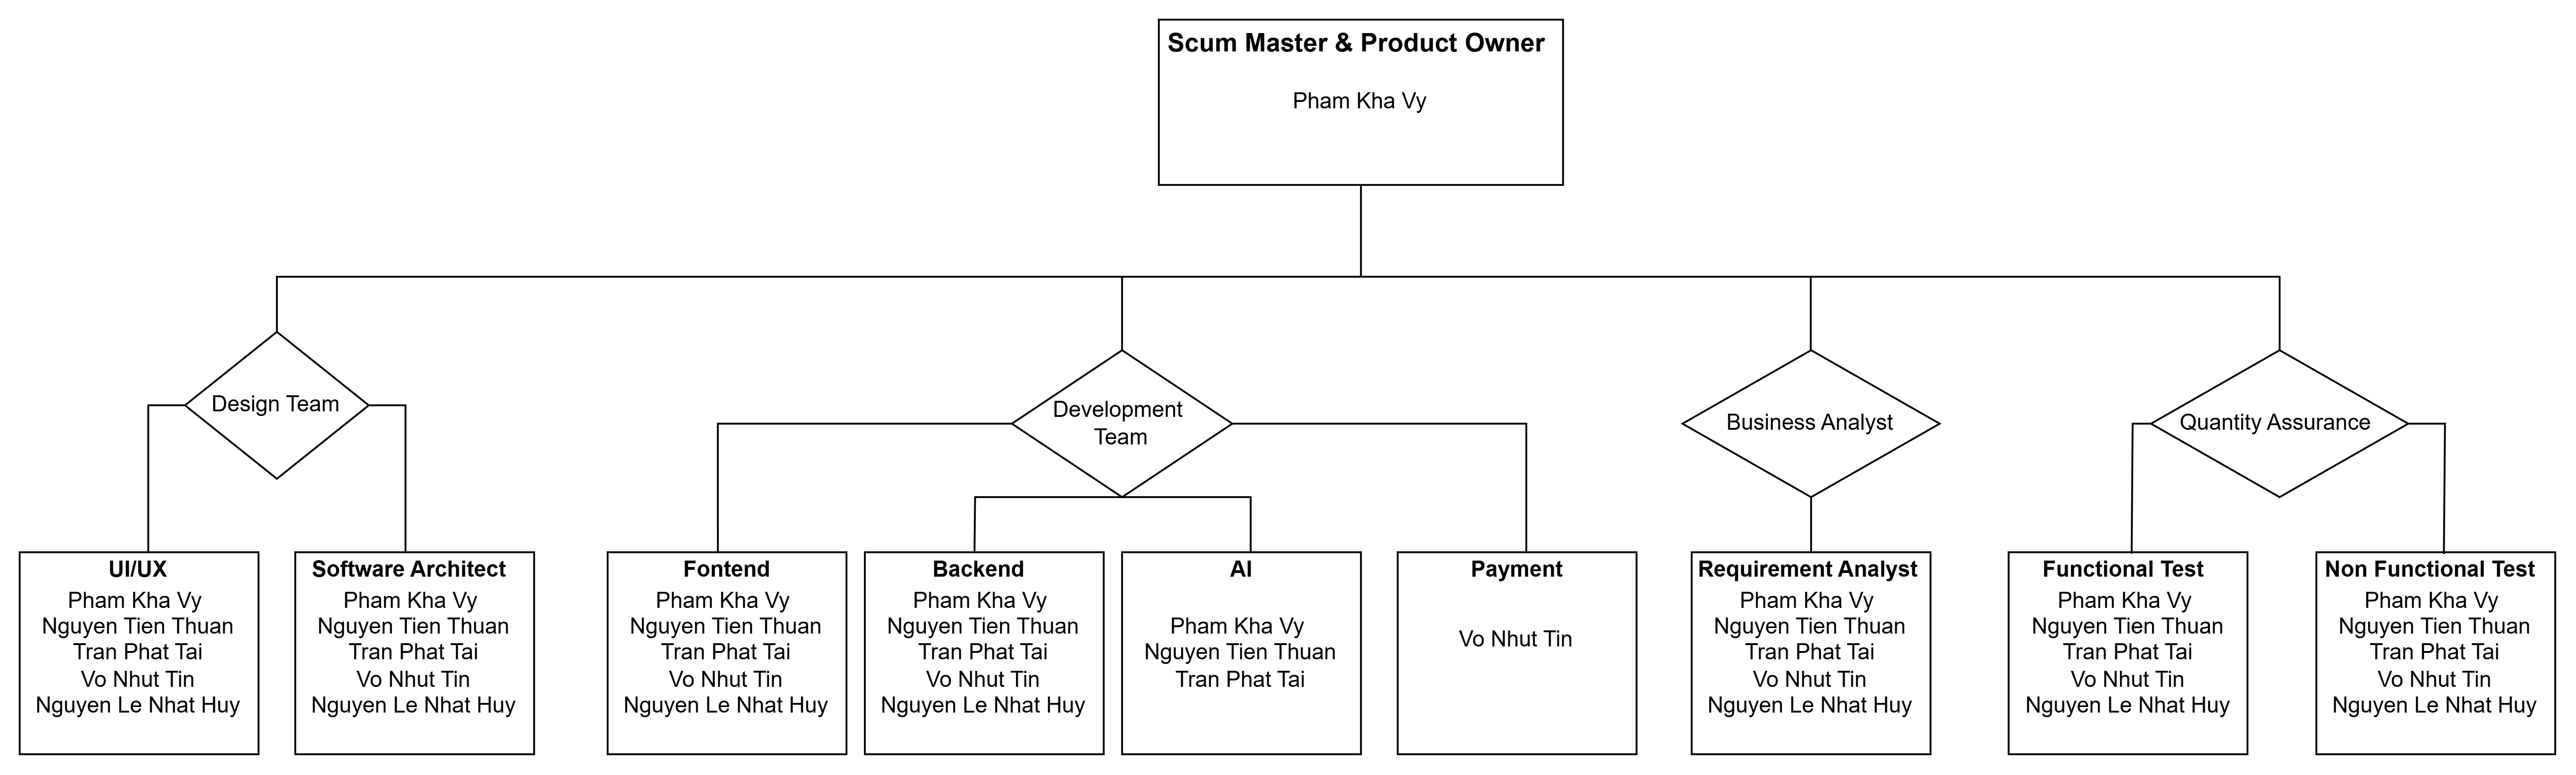
\includegraphics[width=0.8\textwidth]{team-structure.jpg}
\caption{Team and Structure Diagram}
\label{fig:team-structure}
\end{figure}


    \subsection{Role \& Responsibilities}
    \renewcommand{\arraystretch}{1.5}

\begin{table}[H]
\centering
\begin{tabular}{|p{3.8cm}|p{9.6cm}|}
\hline
\rowcolor{headerbg}
\textbf{Role Name} & \textbf{Description} \\
\hline

Product Owner &
Owns the product direction, orders the backlog by business value and dependency, and accepts or rejects each increment at the Sprint Review. In this project the role is combined with the team leader.
\\ \hline

Scrum Master &
Facilitates the Scrum events, protects the sprint commitment from unplanned work, tracks the burndown, and removes blockers that the team cannot resolve on its own.
\\ \hline

UX/UI Designer &
Defines the user flows for the client, freelancer, expert, and administrator journeys, produces the interface designs, and maintains the shared component library used by the web client.
\\ \hline

Software Architect &
Defines the module boundaries of the monorepo, the data model, the contract and milestone state machines, the permission model, and the standards that a change must satisfy before it is merged.
\\ \hline

Frontend Developer &
Implements the Next.js application: routing, forms, data fetching, bilingual message catalogues, and the interface states for loading, empty, error, and permission-denied conditions.
\\ \hline

Backend Developer &
Implements the NestJS modules: controllers, services, repositories, validation schemas, guards, and the database migrations that support them.
\\ \hline

AI Integration Developer &
Integrates the two external AI services that the platform depends on -- curriculum vitae analysis and identity document verification. Defines the request contract, the timeout and error behaviour, the validation of returned data, and the manual fallback used by administrators when a service is unavailable. No model is trained in this project.
\\ \hline

Payment Integration Developer &
Owns the Stripe integration: Connect Express onboarding, platform fee and milestone funding through PaymentIntent and Checkout Session, transfers on release, refunds, dispute fees, settlement, webhook verification, and reconciliation of the transaction ledger against Stripe.
\\ \hline

Requirement Analyst &
Bridges the stakeholders and the development team: elicits requirements, writes the use cases and acceptance criteria, and keeps the requirement specification consistent with what has actually been delivered.
\\ \hline

Functional Tester &
Verifies each delivered item against its acceptance criteria, writes and maintains the test cases, reproduces reported defects, and confirms fixes before an item is demonstrated at the Sprint Review.
\\ \hline

Non-Functional Tester &
Evaluates quality attributes rather than features: authorisation bypass attempts, input validation, response times on list endpoints, behaviour under concurrent messaging sessions, and the stability of the deployment.
\\ \hline

Release and Environment Engineer &
Maintains the containerised development environment, the environment variable contract, the secret provisioning through Infisical, the migration procedure, and the deployment checklist used at the end of each sprint.
\\ \hline

\end{tabular}
\caption{Roles and Responsibilities}
\label{tab:roles_responsibilities}
\end{table}


\section{Project Deliverables}
\renewcommand{\arraystretch}{1.2}

\small

\begin{longtable}{|c|p{6.2cm}|c|c|c|}
\hline
\rowcolor{headerbg}
\textbf{\#} &
\textbf{Deliverable} &
\textbf{Duration} &
\textbf{Sprint} &
\textbf{Week}
\\ \hline
\endfirsthead

\hline
\rowcolor{headerbg}
\textbf{\#} &
\textbf{Deliverable} &
\textbf{Duration} &
\textbf{Sprint} &
\textbf{Week}
\\ \hline
\endhead

\hline
\endfoot
\hline
\endlastfoot

1 & Product Introduction Document & 7 days & Sprint 1 & Week 1 \\ \hline
2 & Project Management Plan & 7 days & Sprint 1 & Week 2 \\ \hline
3 & Software Requirements Specification & 8 days & Sprint 1 & Week 3 \\ \hline
4 & Software Design Specification & 8 days & Sprint 1 & Week 4 \\ \hline
5 & Increment 1: identity and access, profiles, job marketplace, forum foundation & 18 days & Sprint 1 & Week 1--4 \\ \hline
6 & Sprint 1 review and retrospective & 1 day & Sprint 1 & Week 4 \\ \hline

7 & Increment 2: proposals, contracts, milestones and submissions & 14 days & Sprint 2 & Week 5--7 \\ \hline
8 & Updated SRS and SDS (iteration 2) & 2 days & Sprint 2 & Week 6 \\ \hline
9 & Test cases for proposal, contract and milestone flows & 3 days & Sprint 2 & Week 7 \\ \hline
10 & Sprint 2 review and retrospective & 1 day & Sprint 2 & Week 7 \\ \hline

11 & Increment 3: real-time messaging, notifications, administration and moderation & 14 days & Sprint 3 & Week 8--10 \\ \hline
12 & Updated SRS and SDS (iteration 3) & 2 days & Sprint 3 & Week 9 \\ \hline
13 & Test cases for messaging, moderation and identity review & 3 days & Sprint 3 & Week 10 \\ \hline
14 & Sprint 3 review and retrospective & 1 day & Sprint 3 & Week 10 \\ \hline

15 & Increment 4: Stripe escrow, disputes, banners and catalogues & 14 days & Sprint 4 & Week 11--13 \\ \hline
16 & Updated SRS and SDS (iteration 4) & 2 days & Sprint 4 & Week 12 \\ \hline
17 & Stripe test-mode integration suite and webhook scenario tests & 3 days & Sprint 4 & Week 13 \\ \hline
18 & Sprint 4 review and retrospective & 1 day & Sprint 4 & Week 13 \\ \hline

19 & Increment 5: AI curriculum vitae analysis, expert directory, social features and localisation & 14 days & Sprint 5 & Week 14--16 \\ \hline
20 & Quality hardening and full regression run & 4 days & Sprint 5 & Week 15 \\ \hline
21 & User acceptance testing and defect fixing & 5 days & Sprint 5 & Week 15--16 \\ \hline
22 & Deployment package and environment guide & 2 days & Sprint 5 & Week 16 \\ \hline
23 & Final project report & 5 days & Sprint 5 & Week 16 \\ \hline
24 & Thesis presentation and live demonstration & 3 days & Sprint 5 & Week 16 \\ \hline
25 & Updated SRS and SDS (final revision) & 2 days & Sprint 5 & Week 16 \\ \hline

\caption{Project Deliverables}
\label{tab:deliverables}
\end{longtable}

The increments are cumulative. Increment 2 assumes that jobs and profiles from Increment 1 already exist, Increment 3 assumes that contracts and milestones already exist, Increment 4 assumes that a funded milestone already exists, and Increment 5 assumes that the freelancer profile and the verification record already exist. Document deliverables are produced once and then revised at each iteration instead of being rewritten, which is why the SRS and the SDS appear four times in the table.


\section{Responsibility Assignments}
\renewcommand{\arraystretch}{1.3}

\textit{R = Responsible;\;
A = Accountable;\;
C = Consulted;\;
I = Informed}

\vspace{0.3cm}

\small

\begin{longtable}{|p{5.6cm}|c|c|c|c|c|}
\hline
\rowcolor{fptOrange}
\textbf{Responsibility}
&
\textbf{VyPK}
&
\textbf{ThuanNT}
&
\textbf{TaiTP}
&
\textbf{TinVN}
&
\textbf{HuyNLN}
\\ \hline
\endfirsthead

\hline
\rowcolor{fptOrange}
\textbf{Responsibility}
&
\textbf{VyPK}
&
\textbf{ThuanNT}
&
\textbf{TaiTP}
&
\textbf{TinVN}
&
\textbf{HuyNLN}
\\ \hline
\endhead

\hline
\endfoot
\hline
\endlastfoot

Project initiation, scope and risk planning
& RA & CI & CI & CI & CI \\ \hline

Product Introduction Document
& RA & CI & CI & CI & CI \\ \hline

Project Management Plan
& RA & CI & CI & CI & CI \\ \hline

Requirements gathering and user stories
& A & R & R & CI & CI \\ \hline

UI/UX prototype and component library
& A & CI & R & CI & R \\ \hline

Software architecture and data model
& A & R & R & R & R \\ \hline

Authentication, permissions and session management
& A & R & CI & CI & C \\ \hline

Profile, skills, portfolio and curriculum vitae handling
& A & C & CI & R & R \\ \hline

Job marketplace, bookmarks and saved search
& A & C & R & CI & R \\ \hline

Proposal and hiring workflow
& A & C & R & CI & C \\ \hline

Contract signing, milestones and submissions
& A & R & C & CI & R \\ \hline

Stripe escrow, release, refund and reconciliation
& A & C & CI & R & CI \\ \hline

Dispute arbitration and settlement
& A & R & C & C & CI \\ \hline

Real-time messaging and notifications
& A & R & CI & C & R \\ \hline

Forum, moderation and content administration
& RA & CI & C & CI & R \\ \hline

AI integration: identity verification and CV analysis
& A & C & CI & R & CI \\ \hline

Administrative console, catalogues and banners
& RA & C & CI & CI & R \\ \hline

Frontend development
& A & CI & R & CI & R \\ \hline

Backend development
& A & R & R & R & CI \\ \hline

Unit testing
& A & R & C & R & C \\ \hline

Integration and end-to-end testing
& A & C & R & R & R \\ \hline

Payment and webhook security testing
& A & C & CI & R & CI \\ \hline

User acceptance testing
& RA & I & I & I & I \\ \hline

Technical training
& RA & R & R & R & R \\ \hline

Deployment and environment configuration
& A & R & CI & R & CI \\ \hline

Final project report
& RA & R & R & R & R \\ \hline

Thesis presentation
& RA & R & R & R & R \\ \hline

\caption{Responsibility Assignments Matrix}
\label{tab:raci}
\end{longtable}

\normalsize

Accountability is not shared on any row: exactly one member is accountable for each responsibility, and that member is the one who reports its status at the Sprint Review. Where a row lists several responsible members, the work is split by module rather than duplicated, and the split is recorded on the task board before the sprint begins. The rows that carry the highest technical risk -- Stripe escrow and reconciliation, dispute arbitration, and AI integration -- pair a responsible owner with at least one consulted member so that a second person can review the implementation.


\section{Project Communications}
Effective communication depends on a fixed cadence and on a single place where decisions are recorded. Every recurring activity below produces an artefact -- a meeting note, a reviewed pull request, an issue, or an updated document -- so that a decision made in a conversation does not have to be remembered by the people who attended it.

\begin{table}[H]
\centering
\begin{tabular}{|p{3.5cm}|p{3.0cm}|p{2.1cm}|p{4.8cm}|}
\hline
\rowcolor{fptOrange}
\textbf{Communication Activity} &
\textbf{Participants} &
\textbf{Frequency} &
\textbf{Purpose} \\
\hline

Daily stand-up &
Development team &
Daily, 15 minutes &
Report progress since the previous stand-up, state the next item, and raise blockers \\
\hline

Backlog refinement &
Development team &
Weekly &
Re-estimate candidate items, split oversized items, and confirm dependencies \\
\hline

Sprint Planning &
Team members, supervisor &
Start of each sprint &
Confirm the sprint goal and the commitment up to the effort cap \\
\hline

Sprint Review &
Team members, supervisor, invited users &
End of each sprint &
Demonstrate the increment on a running environment and collect feedback \\
\hline

Sprint Retrospective &
Development team &
End of each sprint &
Agree at most two process changes and verify the previous sprint's changes \\
\hline

Design and schema review &
Team members, module owner &
Before each high-complexity item &
Agree on the data model, the API contract, and the permission entry before implementation \\
\hline

Pull request review &
Author and at least one reviewer &
Per change &
Check behaviour, error handling, authorisation, and test coverage \\
\hline

Defect triage &
Team members &
Twice per sprint &
Classify defects by severity and assign an owner \\
\hline

Weekly progress report &
Team leader, supervisor &
Weekly &
Report status against the sprint cap, the risk register, and any support required \\
\hline

\end{tabular}
\caption{Project Communication Plan}
\label{tab:communication-plan}
\end{table}

Communication is conducted through Google Meet for synchronous reviews and supervisor meetings, Discord for day-to-day coordination and quick technical discussion, GitHub for code, pull request discussion, and the issue list, and Google Drive for documents, reports, and shared figures. Figma is used for interface design hand-off, where comments on a frame are resolved before the corresponding frontend item is started.

Meeting outcomes are recorded in a short note with the date, the participants, the decisions taken, and the action items with an owner. The note is stored in the shared documentation folder and linked from the task board, so a member who missed the meeting can recover the decision without asking. A decision that changes scope, schedule, or an existing interface is also recorded in the relevant document rather than only in the meeting note, and the change is announced in the next stand-up.


\section{Configuration Management}
    \subsection{Document Management}
    The project documents are managed as versioned artefacts under the \texttt{docs} directory of the same repository that holds the source code. Keeping the documents next to the code means that a change to behaviour and the change to the document that describes it can be reviewed in the same pull request, which is the only reliable way to prevent the specification from drifting away from the delivered system.

The managed documents include:

\begin{itemize}
    \item Product Introduction (Report 1), describing the background, existing systems, business opportunity, product vision, and the feature and limitation lists
    \item Project Management Plan (Report 2), describing scope and estimation, objectives, risks, organisation, deliverables, communication, and configuration management
    \item Software Requirements Specification (Report 3), containing the actors, use cases, and sprint mapping
    \item Software Design Specification, containing the module structure, data model, and state machines
    \item Test cases and test reports for each iteration
    \item User guide and deployment guide
    \item Meeting minutes and decision notes
\end{itemize}

Documents are written in LaTeX and stored as source files with their figures in a local \texttt{image} directory, so that a document can be rebuilt and diffed rather than being edited as a binary file. The PDF submitted at the end of an iteration is exported from the same source, and the export is repeated whenever the source changes.

Versions follow a two-level scheme: the minor number increases for a review draft or a correction that does not change scope, and the major number increases when a baseline is approved and the document is submitted. A document therefore moves from 0.1 to 0.2 while it is being reviewed, and to 1.0 when it is submitted, and the version and the date appear on the cover page of every submission.

Change control is applied to the Project Management Plan only. A change to the scope, the sprint allocation, the effort estimate, or the deliverables requires an update to the plan together with a short note describing what changed and why. Documents that describe the product rather than the plan are revised freely, because their purpose is to remain accurate rather than to remain stable.

Obsolete versions are retained rather than deleted so that a reviewer can reconstruct what was agreed at a given submission. Each archived version keeps an explicit version suffix in its file name, so that two exports of the same document can never be confused.


    \subsection{Source Code Management}
    Source code is managed in a single monorepo versioned with Git and hosted on GitHub. The repository contains the API application, the web application, the shared packages, the database schema, and the documentation, which allows a change that spans the frontend, the backend, and a shared validation schema to be reviewed and merged atomically.

The following branching strategy is applied:

\begin{itemize}
    \item \texttt{main}: the stable branch. It is updated only at the end of a sprint, from \texttt{develop}, after the increment has been demonstrated at the Sprint Review.
    \item \texttt{develop}: the integration branch. Every member integrates into this branch, and it is expected to build and pass the test suite at all times.
    \item \texttt{uc-[id]-[action-name]}: short-lived feature branches created from \texttt{develop} for a single use case, for example \texttt{uc-09-sign-contract}.
    \item \texttt{hotfix/[short-description]}: urgent corrections created from \texttt{main}, merged back into both \texttt{main} and \texttt{develop} so that the fix is not lost at the next integration.
\end{itemize}

A change is merged only through a pull request. The pull request must reference the SMAR identifier it implements, describe the behaviour that changed, and state how it was verified. At least one other member must approve it, and the author may not approve their own change. The project's Definition of Done is applied at review time: the lint, type-check, and test commands pass, the container build succeeds, the new endpoint is registered in the permission model, and the user-facing text exists in both language catalogues.

Commit messages are written in the imperative mood with a short scoped summary, so that the history of a module can be read without opening the diff. A commit that changes the database schema is separated from the commit that changes application behaviour, which makes a migration easy to identify and to revert independently.

Direct pushes to \texttt{develop} and to \texttt{main} are not permitted, and neither branch may receive a force push after it has been shared. Branches are deleted after merge so that the branch list reflects only work that is in progress.

Generated artefacts are excluded from version control: build output, dependency directories, uploaded files, coverage reports, and environment files. Secrets are never committed; configuration is supplied through environment variables loaded from the secret manager described in Section 7.3, and the committed environment template contains only the names of the variables and placeholder values.

The repository layout mirrors the architecture: \texttt{apps/api} contains the NestJS application with its Prisma schema and migrations, \texttt{apps/web} contains the Next.js application, \texttt{packages/shared-type} contains the Zod schemas and the types derived from them, \texttt{packages/ui} contains the shared interface components, and \texttt{docs} contains the reports and the specifications. The deployment definition, the workspace configuration, and the task pipeline live at the repository root so that a fresh clone can be started with a single command.


    \subsection{Tools \& Infrastructures}
    \begin{table}[H]
\centering
\begin{tabular}{|p{3.5cm}|p{9.9cm}|}
\hline
\rowcolor{fptOrange}
\textbf{Category} & \textbf{Tool} \\
\hline
Project tracking & GitHub issues, milestones, and the project board in the same repository as the code \\
\hline
Version control & Git with GitHub; two long-lived branches and short-lived use-case branches \\
\hline
Communication & Discord for daily coordination, Google Meet for reviews and supervisor meetings \\
\hline
Documentation & LaTeX sources in the repository, Google Drive for shared material, Microsoft Word where a form is required \\
\hline
UI/UX design & Figma \\
\hline
Runtime and workspace & Node.js with pnpm workspaces and Turborepo task orchestration \\
\hline
Frontend & Next.js 16 App Router, React 19, Tailwind CSS 4, the shared component library, next-intl for English and Vietnamese, TanStack Query for server state, Tiptap for the forum editor \\
\hline
Backend & NestJS 11 with a global API prefix, Zod validation through nestjs-zod, a permission guard, and Socket.IO for messaging \\
\hline
Data access & Prisma 7 with the PostgreSQL driver adapter; migrations generated from the schema and applied per environment \\
\hline
Database & PostgreSQL \\
\hline
Shared contracts & \texttt{packages/shared-type}, containing the Zod schemas and the types used by both applications \\
\hline
Payments & Stripe, in test mode throughout development: Connect Express, PaymentIntent, Checkout Session, transfers, refunds, and a signature-verified webhook \\
\hline
Media storage & Cloudinary for profile and portfolio images; identity documents stored on the application's own storage and served through authenticated endpoints \\
\hline
Email & SMTP through Nodemailer for one-time verification and password reset codes \\
\hline
External AI services & A curriculum vitae analysis service and an identity verification service, both called only from the backend over HTTP with an explicit timeout \\
\hline
Testing & Jest 30 for unit and integration tests, an end-to-end test against the running API, and Postman for exploratory API checks \\
\hline
Quality tooling & ESLint 9 and Prettier, plus the TypeScript compiler in strict mode through the shared configuration package \\
\hline
Secret management & Infisical, injecting environment variables at start-up; no secret is stored in the repository \\
\hline
Containerisation & Docker with Docker Compose, providing the API and the web client; the API exposes a health check and the web client starts only after the API is healthy \\
\hline
API documentation & A maintained reference in the repository describing each endpoint, its permission, and its request and response schemas \\
\hline
\end{tabular}
\caption{Tools and Infrastructures}
\label{tab:tools}
\end{table}

The tool selection follows a single constraint: a member must be able to reproduce the whole system from a fresh clone with one command. That is why the runtime, the database, the task pipeline, and the container definition are all pinned in the repository rather than installed manually per machine. It is also why the configuration is injected through a secret manager instead of being copied between members, and why the API reference is kept in the repository rather than in a separately hosted portal.

Two capabilities are deliberately not part of the toolchain. There is no automated continuous integration service: the same quality gate is executed locally and inside the container build, and the reviewer confirms the result before approving a pull request. There is no hosted API documentation portal; the reference is a maintained document, which is sufficient for a team of five and avoids a second source of truth that can fall out of date.


\end{document}
